\documentclass[a4paper, 12pt, openany, oneside]{book}
% Header file
% author: marcobecerrap
% date: January-2015

\usepackage{cite} % Citation Package
\usepackage{natbib} % Citation style
\usepackage{graphicx} % Graphics Package
\usepackage{amssymb, amsmath, amsbsy} % Equations
\usepackage{caption}
\usepackage{subcaption}
%\usepackage[utf8]{inputenc} % Special characters (e.g. spanish accents).
\usepackage{pgfgantt} % Gantt Charts
\usepackage{lscape} % Included packages located in a separate file
\pagestyle{plain} %Page numbers on the bottom

\begin{document}

% Front page
%\pagestyle{emty} %No numbers
%%\begin{titlepage}
%\begin{center}
%	{UoB, CS}\\
%	{Report 3}\\
%	{Title: SM of HE with a MR}\\
%	{Student: MABP}\\
%	{Supervisor: NH}\\
%	{Thesis Group: JW PH}
%\end{center}
%\end{titlepage}


\begin{titlepage}
\begin{center}

   {\Large \textsc{University of Birmingham}}
	\vskip 10pt
	{\Large \sc School of Computer Science}

%\vskip 0pt plus 2fill
\vspace{50pt}
{\Huge\bf Thesis proposal }\\
\vspace{40pt}
\includegraphics[width=6cm]{fig/uob_coat.pdf}
%\pgfdeclareimage[width=8.5cm]{logo}{fig/logo_cvut}
%\pgfuseimage{logo}

\vspace{40pt}
{\Large\rm Marco Antonio Becerra Pedraza} \\
\vspace{20pt}
{\Large\bf Semantic Mapping of Human Activities}\\
\vspace{0.2cm}
{\Large\bf with a Mobile Robot}\\

\vspace{40pt}
{\bf Intelligent Robotics Lab}\\
\vspace{5pt}   
{Supervisor: {\bf Dr. Nick Hawes}}\\
\vspace{5pt}   
{Thesis group members: {\bf Prof. Jeremy Wyatt, Dr. Peter Hancox}}
\vfill 
{Birmingham, 26.3.2015}
\end{center}
\end{titlepage}
%\cleardoublepage

% Table of Contents
%\newpage
%\pagenumbering{roman}
%\tableofcontents

% Main Chapters
\newpage
\pagestyle{plain}
\pagenumbering{arabic}
% Abstract
%\chapter{Introduction}

% INTRO 
% > Robots in everyday environments are important.
% > This environment is hard.
% > Robots needs cognitive skills: understand the environment.
\section{Introduction}
One of the main goals in AI is having robots working autonomously in everyday environments. 
In such situation, robots are expected to perceive, understand and interact with its environment. 
However, these kind of environments are dynamic, non-structured and non-deterministic, which makes difficult for a robot to fulfil the assigned tasks. 
To be able to sort these obstacles, robots need to be provided with cognitive skills.

Human cognition refers to all mental activities associated with thinking, knowing, remembering and communicating, and how the information is processed \citep{King2014Psychology,myers2013psychology}. 
In robotics, the concept is associated with systems that emulate these mental processes or those that \textit{sense}, \textit{plan} and \textit{act}.
More precisely, cognition can refer to those systems that can perceive, understand \ldots and interact with their environment, and evolve in order to achieve human-like performance in activities requiring context (situation and task) specific knowledge \citep{christensen2010cognitive}.

% GENERALITIES ABOUT HUMAN ACTIVITIES
% > Activities are important part of the scenes and they are necessary to be able to understand the scene
% > Activities are entities with a spatio-temporal & symbolic (semantic, hierarchical) characteristics
Everyday environments have many valuable features that a robot needs to understand, in order to succeed while performing a task, among them are human activities.
Human activities are a meaningful manifestation of human behaviour along time and space. %TODO Expand the definition of activity.
They provide rich information about the human performing it, but also, about his/her relation with other relevant components of the environment as humans, objects and locations.


%\section{Research Problem}
\subsection{Human activity analysis with a mobile robot}
% ACTIVITY RECOGNITION
% > AR as a field
% > Robot case, advantages and disadvantages of using a robot
Activity recognition is the research field that studies the automatic detection and analysis of human activities by processing the data acquired from sensors \citep{Aggarwal14_HumActRec3DRev}. 
It is not restricted only to sensory data and this can also be complemented with other sources of information, i.e. domain knowledge.
In the AI context, activity recognition is closely related with the areas of perception, knowledge representation and reasoning. 
The problem of activity recognition has been treated from different perspectives, however, computer vision has been the most popular.

% Robots in AR (general)
In principle, robots with appropriate sensing and processing capabilities can perform activity recognition. 
Moreover, they have some advantages over the use of fixed cameras or wearable devices as they are able to interact with the environment. 
Robots are active observers, i.e. they can change their point of view on scene and be selective in the areas of the environment that are more interesting. 
On the other hand, they have some disadvantages as well. 
They don't have omnipresence, so they are not able to sense the full environment and will loose information.
Also, their sensors have constraints, the data may be noisy or blurry due to movement, erratic hardware, changing environmental conditions, etc. 
Finally, robots are expected to work in real-time, so online activity recognition is desirable but yet difficult to achieve.

% BRIDGE TO ASP
Activities involve knowledge.
They associate concepts and relations between a subject and the environment.
In general, an activity recognition system should be able to handle, not only sensory data but also symbolic representations, and be able link top level symbolic concepts to low level sensory data; this is known as the \textit{anchoring problem} \citep{Coradeschi03_AnchoringProblem}.
With this in mind, knowledge processing and reasoning is a necessity for such systems.


\subsection{Answer Set Programming for Knowledge Representation and Reasoning}

There have been proposed many ideas to handle the problems of knowledge representation and reasoning (e.g. logic programming, ontologies, bayesian networks, fuzzy logic, etc.), among them is Answer Set Programming (ASP).
ASP is form of declarative programming oriented towards difficult, primary NP-hard, search problems.
It establish a new paradigm of logic programming that allows concepts as negation as a failure, default knowledge and non-monotonic reasoning.

ASP main concepts were proposed since the late 1980s \citep{Gelf88a} and it has been used with success in many applications.
Traditionally, ASP solvers were designed as one-shot problem solvers, so they lacked of reactive capabilities and, for example, whenever new data arrived, the system needed to be restarted.
This has been one of the main reasons why ASP has not been fully exploited in the field of robotics, however, in recent years an important effort has been directed towards this direction by some groups \citep{AndresOSSR13_rosoclingo,Erdem2013_IntLowRTaskP}.


\section{Research Problem}

This project is based in the consideration of ASP as a solid option for robots in problems that require symbolic representations.
The focus of this project is to study \textbf{ASP-based activity recognition with a mobile robot}. The interest lies  in the spatio-temporal relation between human activities and the environment and how a robot can acquire, handle and use this knowledge.

ASP allows the manipulation of incomplete information and handling multiple sources of knowledge.
The integration between observations and external knowledge appear to be a more robust approach than a single sensory based approach.
Hardware adds uncertainty via noise, is constrained by its specification and the outcome data is usually difficult to process.
This uncertainty cannot be eradicated in robots, but the treatment of some problems as activity recognition can be boosted by emphasizing a more cognitive approach. 
%(via) the it can be  by emphasizing cognitive mechanisms By putting emphasis in the cognitive essence of the problem of activity recognition, the uncertainty in the cognitionemphasizing aputting emphasis in athe upper layer of knowledge representation and reasoning in solving problems that require cognition, the system would rely totally onenable, not to eradicate, but to complement a sensory based approach and also to minimize its charge in a system.

\subsection{Expected outcome}

The expected outcome will be a systematic analysis of ASP-based activity recognition and its use with a mobile robotic platform.

First, the problem of activity recognition will be treated via ASP and compared with other state-of-the-art approaches.

Experience acquisition will be studied via semantic mapping to progressively create a knowledge source for a robot regarding the activities occurring in a particular location and that can be used by the robot for future inferences.

Finally, we are interested in taking advantage of the activeness of the robot to improve the perception and knowledge acquisition processes in the context of activity recognition; e.g. looking for missing information, the ability to get information from the environment more efficiently, etc.



% RESEARCH PROBLEM
% > Talk about AR with a robot in cases with incomplete information
% > Generalities of the problem 
% > Example case of a sequence
%TODO %TODO %TODO %TODO %TODO %TODO %TODO %TODO %TODO %TODO %TODO %TODO %TODO %TODO %TODO %TODO

%Persentation of the project
%Particularly in the case where there is not complete information from the environment to have a clear match between the observations and %the activity patterns. 
%Here, an interpretation can still be made using previous experience and domain knowledge. 
%Even, if a totally certain interpretation of the scene is not possible, a partial one can still be done with a list of the most probable situations to be happening. 
%This also can be used by a robot to decide to perform new observations of the scene to improve its reasoning conclusions. 
%The chosen technique to do this is Answer Set Programming (ASP).

%TODO Write paragraph about ASP
%Answer Set Programming is a logical p

% Quick draft of the proposal.

\section{Test scenario: ``The library setting''} \label{sec_Library} %TODO Add images.

Because human activities cover a broad range o possible situations, it becomes a necessity to bound the scope of this project and look into exemplar cases that can be used to demonstrate the ideas. 
With this in mind, it has been chosen a library as a scenario to test and explain the ideas of this project.

The School of Computer Science at the University of Birmingham has a library, Fig. \ref{fig_library}.
The physical scenario is basically a big room. 
It has some cabinets (where bibliographic material is stored), a reception desk, some tables with chairs and a printing area. 
It has only one entrance.
An attendant is in charge of the book loans and retrievals, and also to assist the users.
Most users use the facility to study, to consult material, to print, for team work, to use their laptops or simply as a rest area.

%TODO Add images (1) real library, (2) Lars SemMap
\begin{figure}[tbp]
  \centering
  \subfloat[Real library]{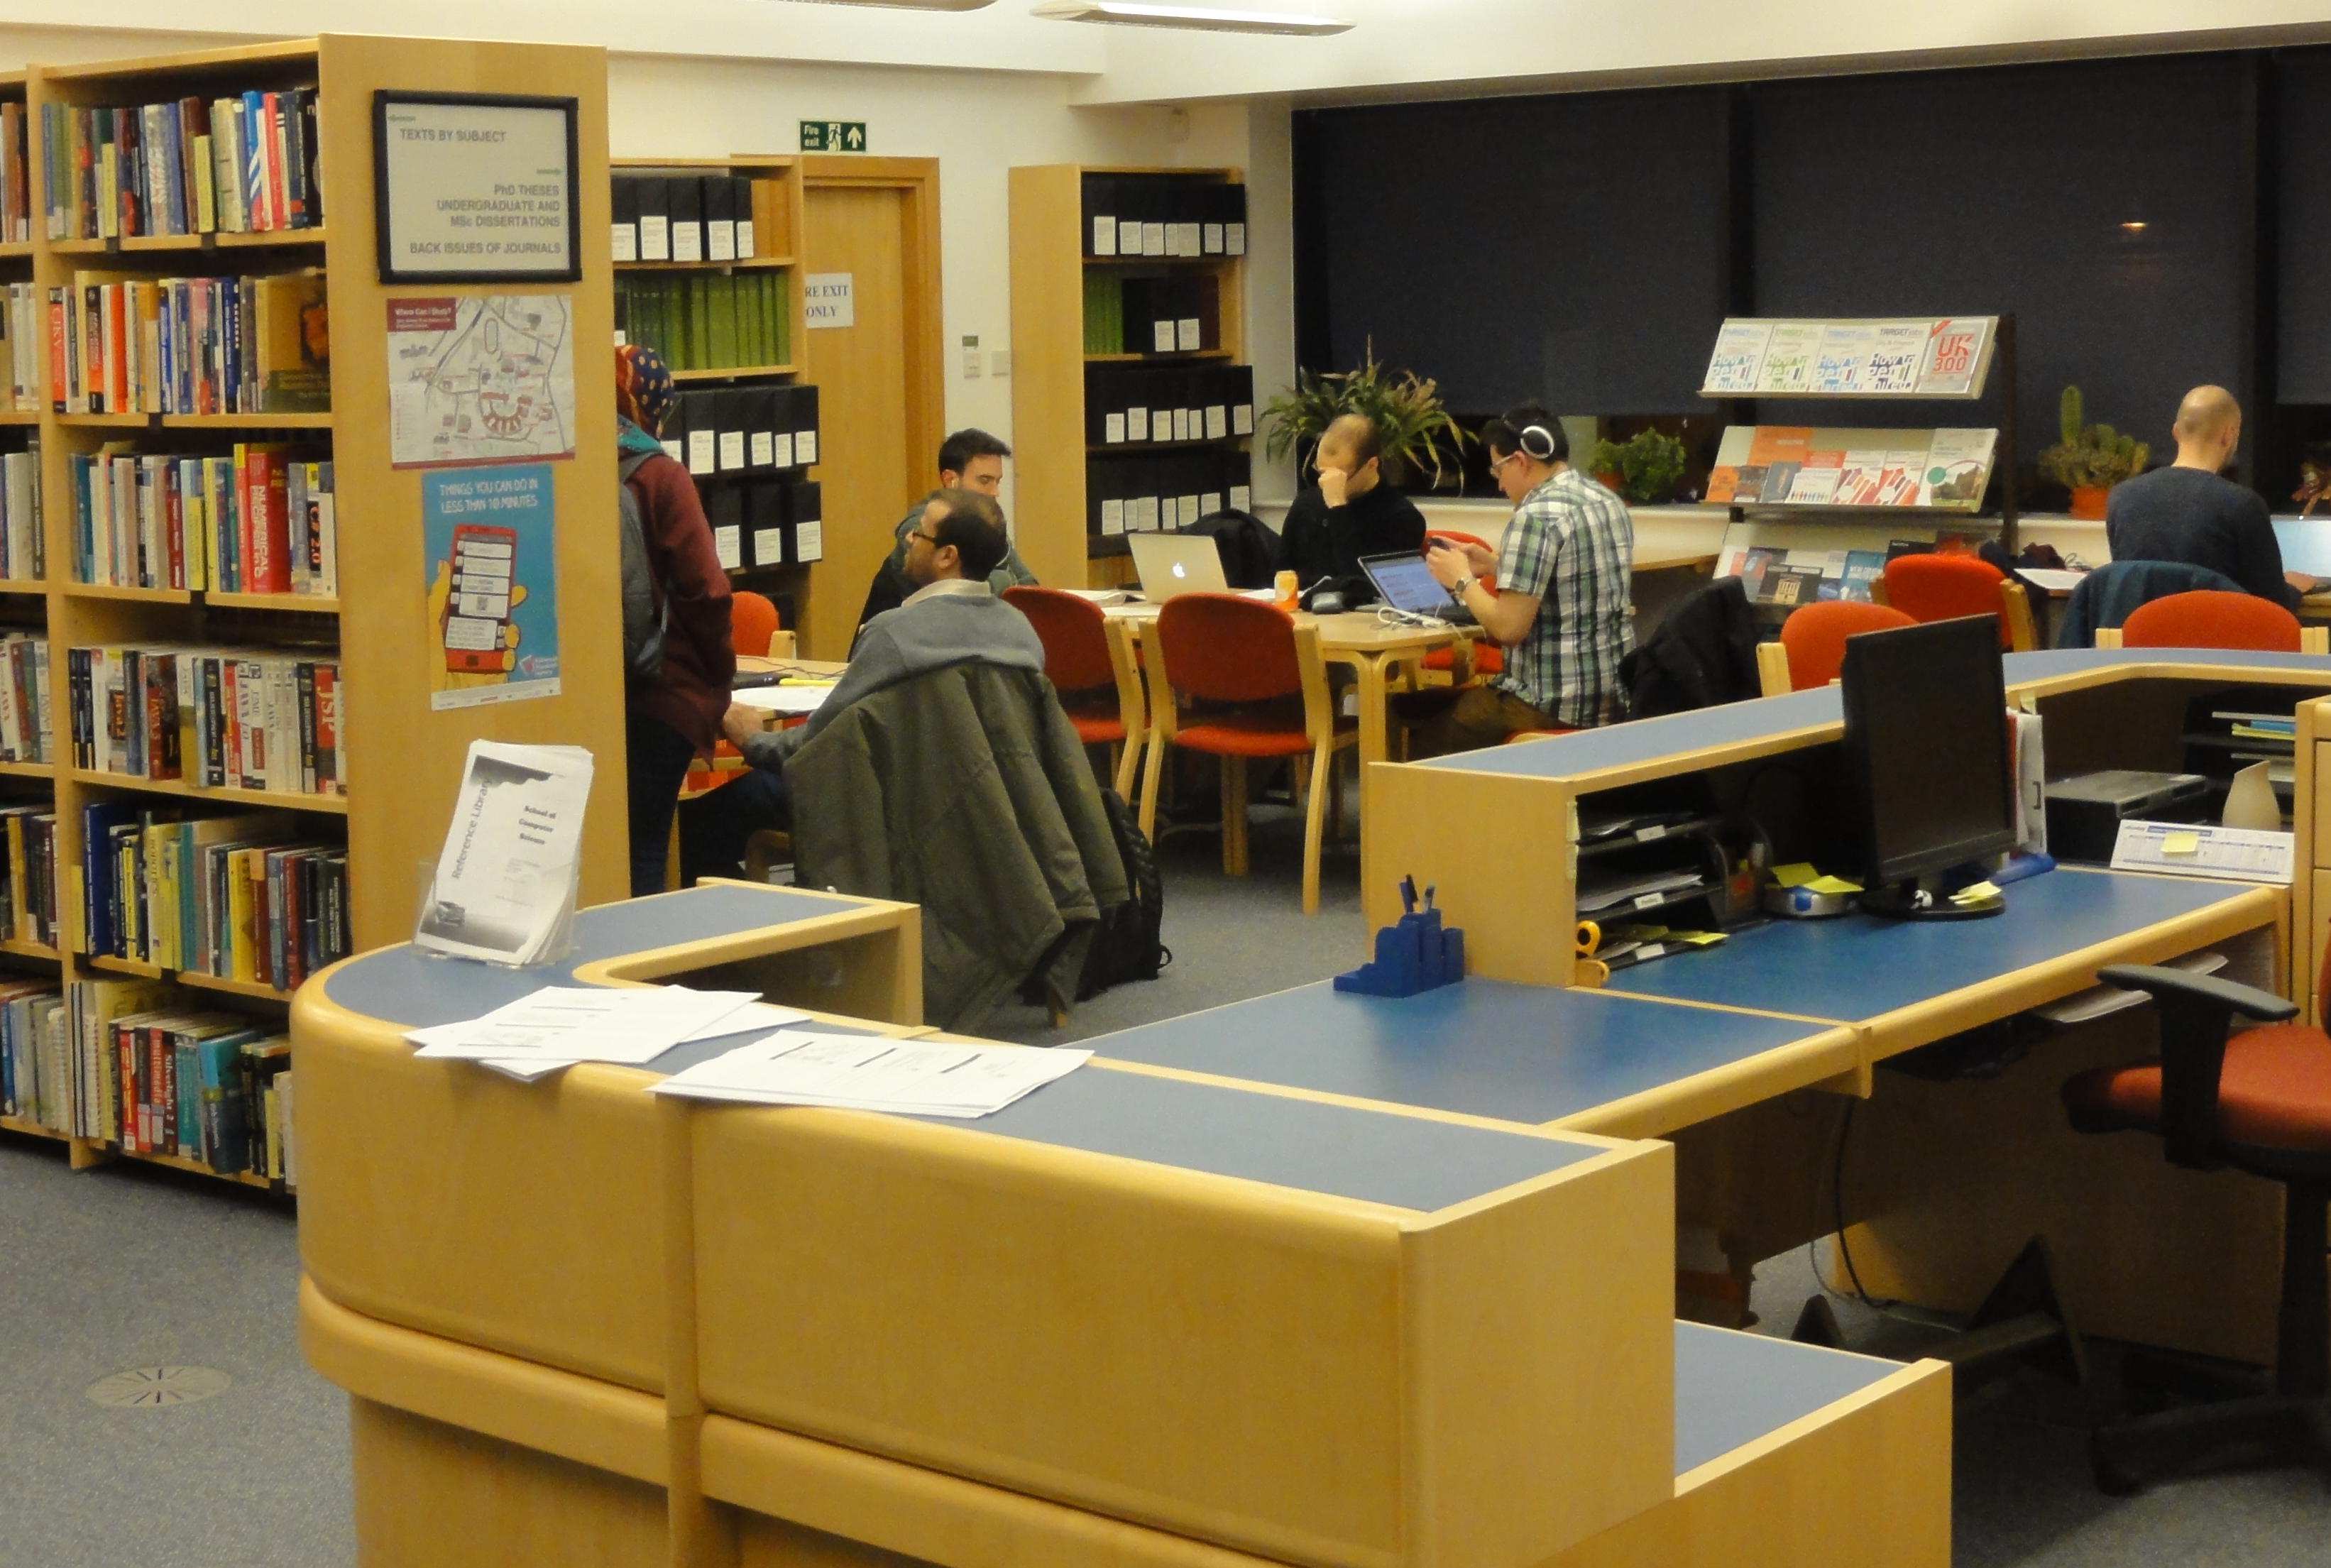
\includegraphics[width=2.5in]{fig/Library02.png}}\quad
  \subfloat[Semantic map of the library]{\includegraphics[width=2.5in]{fig/Library01.png}}\\
  \label{fig_library}\caption{The library setting}
\end{figure}

Because of the rules of the library and the nature of the location, the amount of activities is limited.
However, non-considered activities could eventually appear, as giving a greet, using a cellphone, talking, etc.
The amount of objects involved in the environment is also relatively small (books, tables, chairs, laptops, cabinets, etc.).

Our interest is to use this library setting as a test for activity recognition with a mobile robot, and moreover
The problem can be analysed with simple examples via simulation to build the core of a testing system, and later use real data and eventually a mobile robot.
%Libraries tend to share some similarities, there is the possibility to replicate the experiments from this work in other locations.
%This would create landmarks for testing and comparing different approaches, and direct the research towards a more general and better system.

%For the sake of simplicity and as a starting point, lets consider the following abstraction: a linear library (Fig. \ref{}).

%\begin{figure}[h]
%\centering
%\includegraphics[width=\textwidth]{fig/img_Aggarwal_Taxonomy2.pdf}
%\caption{The taxonomy of research in activity recognition described in \cite{Aggarwal11_HumanActivity}.}
%\label{fig:taxonomy}
%\end{figure}




%Some interesting activities to look at are:

%\begin{description}
%\item[book loan] A person goes to the reception with a book, spend some time on it and later leaves the library with the book.
%\item[book retrieval] A person arrives to the reception with a book and \textit{leaves} the book in the reception.
%\item[study] A person
%\end{description}


%TODO %TODO %TODO

\section{Document organization}

The rest of the document is organized in the following manner.

Chapter \ref{ch_relatedwork} presents related literature to the problem and discusses the results and limitations of previous approaches. The chapter starts with a brief historic presentation of perception in Artificial Intelligence and goes towards the problem of activity recognition. Section\ref{} presents a summary of how the problem of activity recognition has been treated before, and particularly regarding hierarchical description-based approaches, in which ASP is an alternative. In section \ref{sec_DBROB}, some previous works that integrate activity recognition and robotics are reviewed. Finally, in section \ref{sec_DBROB}, ASP is presented as an alternative for solving problems that require knowledge representation and reasoning.

Chapter \ref{ch_research_problem} presents the problem (section \ref{sec_problem}) and the proposed methodology (section \ref{sec_methodology}) to treat it. 

Chapter \ref{ch_eva} presents an experimental approach to evaluate the methodology proposed within this project. By using variations of the library setting environment (section \ref{sec_Library}), the problem can be studied gradually and the main components of an ASP-based approach can be remarked.

Chapter \ref{ch_wp} presents a work plan for the rest of the project duration (2 years) and proposes goals and tasks to achieve them. 

Finally, chapter \ref{ch_conc} presents the conclusions final comments regarding this project and about the developed ideas.









 % Intro & Motivation (Open areas proposed in the literatures)
\chapter{Introduction}
Presentation of the project.

Current state[60\%].
Goals:-

\section{Human activity Analysis}
Justification of the problem and how this is linked to robotics.
At the same time, these should be linked to the project (ASP).
This is the route from the general problem to my project, described in general here, but with more detail in the next chapter.
Current state[90\%].
Goals: -


\subsection{Test case: ``The library scenario''}
Presentation of the test scenario.
An example is needed here, to introduce an example that the proposed approach can treat.

Current state[70\%].
Goals: Put the problem example here.


\section{Methodology}
The presentation of the project, i.e. proposal in general.

Current state[10\%].
Goals: Present the project. What kind of techniques are going to be used? Why?


\subsection{System presentation}
Structure of the system.
How all parts assemble together.

Current state[10\%].
Goals: Describe in general the project and what kind of system is being proposed. Some proposed experiments.


\subsection{Outcome}
The scope of the project.
Expected challenges and outcome.
Evaluation.


Current state[10\%].
Goals: What challenges and results are expected.


\subsection{Outline}
Outline for the rest of the document (this could be done wwith the structure of the document).


%\chapter{Related Work}

% 0 - GENERALITIES
% Symbol ground
% Anchoring
% Frame Problem


% 1 - ACTIVITY RECOGNITION
% Historic origins
% Main branches
% Hierarchical pproaches


% 2 - ANSWER SET PROGRAMMING
% General background
% Related work to AR


% 3 - ASP + Robots -> ROSoClingo
% 
 % "Related Work" Literature rev (separated areas, in my case AR + ASP + KRR(incomplete) + Semantic Map)
\chapter{Related Work}

Current state[90\%].
Goals: Last section (discussion), I think is needed to link my project in the literature review.


\section{General antecedents - Perception in AI}
This is are the main branches where the problem come from (how has been studied) and especially, from a CS point of view.

\section{Activity Recognition} 
Presentation of the taxonomy of the problem. 
How has been treated before.
What techniques have been used.
The taxonomy is built upon the representation and techniques used.

\subsection{Single-layered approaches}
Analysis of low level actions (usually atomic ones).
\subsubsection{Continuous approaches} % BEFORE: Space-Time approaches
\subsubsection{Sequential approaches} %TODO Go deeper.

\subsection{Hierarchical approaches}
High level activity recognition (symbolic and statistical).
\subsubsection{Statistical}
\subsubsection{Syntactic}
\subsubsection{Description-based} \label{sec_description_ap}

\section{Description-based activity recognition and mobile robotics}
This is the main branch where this project fits.
I go in detail with the techniques that I'm looking at.
I also try to establish the link with robotics.

\subsection{Description-based activity recognition}

\subsubsection{Activity recognition from a robotics perspective}
Previous works in robotics, some that serve as example of the progress, used approaches in the area and uncovers the open problems.

\section{Answer Set Programming} % Because is one of the main contributions, I put it appart.
As this is an important part of my thesis, I present it here in general

\subsection{ASP as a declarative problem solving technique}
What kind of problems can be treated with ASP.
How does it work.
How problems are modeled with ASP.

\subsection{ASP as a knowledge representation language}
Link ASP to knowledge representation.
Some pros & cons, and challenges ahead

\subsubsection{ASP implementations}
Present popular systems around (potassco & DLV).

\subsection{ASP and robotics}
% University of Sabanci
Link ASP with robotics.
R-Sabanci University.
R-Potsdam University.

\section{Discussion}
Conclusions about the state of the art.
What is missing, and how my project fits there.

%\section{Semantic Mapping}



%\chapter{Research Problem}

\section{Human activity analysis}
% Description of the problem

%TODO Main sentence for the problem

The application domain will dictate the activities to be recognized, the required precision, the sensors to be used and their location (environment located or wearable), the time constraints for deliberation,



%The main goal is to automatically analyse the ongoing activities from a sensory source (a video sequence in most of the cases).

%Activities can be understood in physical terms (space and time), but also symbolically as they can usually be associated with a meaning and a context. 

%Human activities are difficult to classify because they cover a broad range of situations and they depend on different parameters.
%Regarding their complexity, activities can be treated as hierarchical entities because high-level activities are usually composed of simpler actions.
Regarding the complexity of the activities, in \citep{Turaga2008_MaRecHuAcSurv}, two non-exclusive categories are used: actions and activities.
The first one is used for simple actions performed preferably by a individual, and activities are treated as a complex sequence of actions performed by several individuals. 
On a similar fashion, in \citep{Aggarwal11_HumanActivity}, a four layers categorization is proposed:

\begin{description}
\item[Gestures] Elementary movements of a person's body part, and are the atomic components describing a meaningful motion of a person. 
E.g. `stretching an arm', `raising a leg'.
\item[Actions] Single person activities that may be composed of multiple gestures organized temporally. 
E.g. `walking', `waving'.
\item[Interacions] Human activities that involve two or more persons and/or objects. 
E.g. `Two persons fighting', `a person eating an apple'.
\item[Group activities] The activities performed by conceptual groups of multiple persons and/or objects. 
E.g. `a football team playing a match', `a group of students making an exam'.
\end{description}









% Alternatives for each part
% > Observations
% > Knowledge (where? & how?, I'll do it by hand, but it's important to mention alternatives).
% > Representations
% *** CHECK THE orgnanization from the surveys
%   - Modelling activities in space (QSR)
%   - Modelling activities in time  (QSTR ~ Allen's, Fluent, Event, etc).
%   - Modelling activities semantically (Ontologies + Hierarchies)
% > Inference

% Test example

\section{Proposal} % Or alternatives

% Main parts of the problem

% A - Scene decomposition (locations, objects, persons)
%   > from observations to scene reconstruction

% B - 

% B - Representation 
% Modelling in space (QSR)
% Modelling in time (QSTR)
 % (Mike --> Model & Methodology) % Research Problem (Analysis) (Problem Definition -> Rafee)
\chapter{Research Problem}
Current state[50\%].
Goals:-

Present the problem, the one for this project.

\section{Description}
Current state[50\%].
Goals: Need to go to the point and connect it with the library example.

Use the library case, the example.
What kind activities are going to be solved?
What kind of data are we inderested in?


\section{Methodology}
Current state[50\%].
Goals: Reuse the diagram from the first chapter and develop it.

What kind of system is going to be used (proposed)?
What do I already have in hand?
What is missing?


\section{Evaluation}
Current state[20\%].
Goals:-

What kind of challenges are expected?
What is the strategy for them?

What kind of outcomes are expected?


\chapter{Work Plan}
Current state[0\%].
Goals: Present the parts of the problem  and how are they going to be assembled. This is the first goal. Then I need target simple test examples. Then focus on improvements. Set goals (e.g. present work).

What's the next step for this project?

Put yourself some goals.

\section{Short term (6 months - 1 year)}
\section{Long term}
\section{Timetable}

\end{document}
